\documentclass[../main.tex]{subfiles}

\begin{document}
Với bài toán nhận diện tên thực thể Y Sinh, mô hình học đa tác vụ, cùng với kiến trúc BiLSTM-CRF là mô hình học sâu được chọn để giải quyết. Đầu tiên, mô hình sẽ sử dụng BiLSTM trên mức kí tự. Bên cạnh đó, embedding của các từ cũng sẽ được cho qua BiLSTM để nắm bắt thông tin ở mức từ ngữ. Kết quả của việc đưa từ và kí tự qua LSTM sẽ được ghép với nhau và đưa đến tầng cuối cùng là CRF. Tầng CRF này sẽ giúp gán nhãn cho chuỗi đầu vào. 

\textbf{Mô hình xử lý một tác vụ:
}
\begin{figure}[h]
\centering
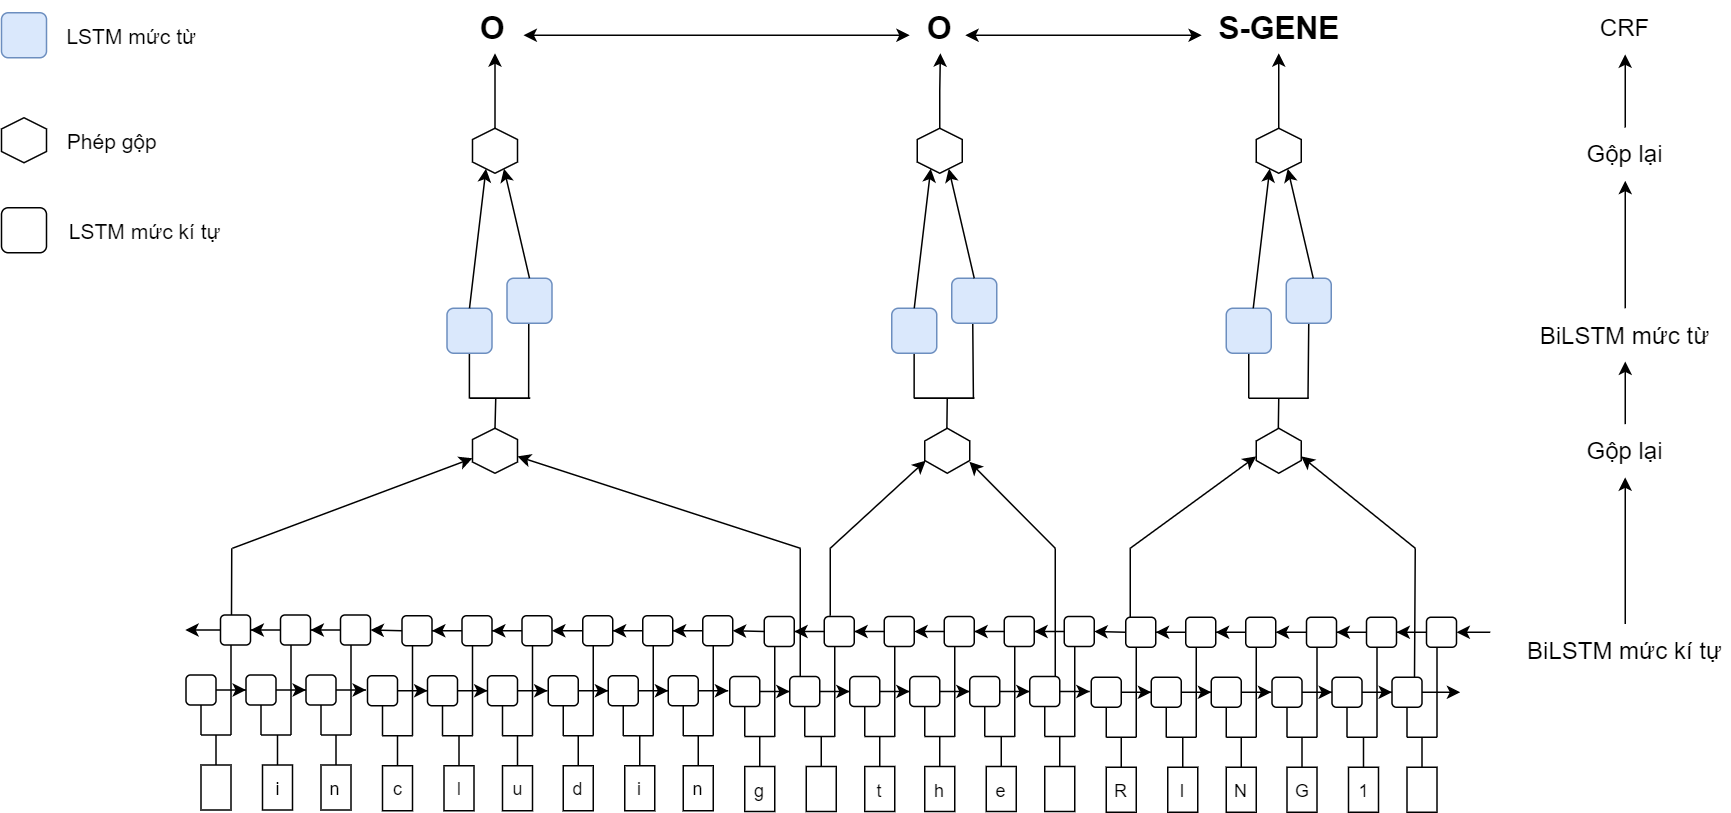
\includegraphics[scale=0.28]{03-BiLSTM-CRF}
\caption{Kiến trúc mạng nơ-ron. Câu đầu vào là từ một văn bản Y Sinh. Các hình chữ nhật mô tả embedding của từ và các kí tự. Hình chữ nhật có viền tròn thể hiện kết quả việc sử dụng BiLSTM trên mức kí tự. Hình chữ nhật viền tròn có màu bên trong thể hiện kết quả việc sử dụng BiLSTM trên mức từ. Hình lục giác thể hiện phép gộp các kết quả lại với nhau. Các nhãn trên cùng là 'O' hay 'S-GENE' thể hiện đầu ra của tầng CRF - là các nhãn của thực thể cho mỗi từ trong một câu}
\end{figure}


\begin{itemize}

\item Word Embedding: 

Với embedding ở mức từ, khóa luận này sử dụng vector cung cấp bởi mô hình BioWordVec - dựa trên tư tưởng của fastText rồi huấn luyện lại trên dữ liệu có miền đặc thù là Y Sinh: \textit{PubMed} và \textit{MIMIC III Clinical notes}. Các vector này có 200 chiều, giúp ánh xạ một từ vào không gian vector các số thực để có thể tính toán được. Ưu điểm của mô hình là giúp sinh ra được biểu diễn của những từ mà chưa từng gặp dựa trên các từ con hình thành bởi $n$ kí tự liên tiếp. Điều này giúp nắm bắt thông tin tối đa về ngữ nghĩa của các từ, trong đó có cả các từ thuộc về tên của một thực thể Y Sinh. 

\item BiLSTM:


Mô hình BiLSTM-CRF có thể học được những biểu diễn có chất lượng tốt cho các từ xuất hiện trong tập huấn luyện. Tuy nhiên, mô hình lại thường thất bại trong việc tổng quát hóa các từ không nằm trong tập từ vựng (out of vocabulary - OOV) vì không có embedding được huấn luyện sẵn. Nhờ thế mà mô hình trong khóa luận này sẽ thêm một mạng BiLSTM để mô phỏng chuỗi kí tự trong câu đầu vào. Đầu vào của mạng là embedding của các kí tự. Sau khi cho qua mạng BiLSTM sẽ tạo ra các vector trạng thái ẩn. Các vector trạng thái ẩn đó tương ứng ở các vị trí biên của mỗi từ sẽ được ghép vào với nhau, sau đó tiếp tục ghép vào với các vector embedding của các từ đã có được ở tầng embedding của từ để tạo thành biểu diễn từ cuối cùng. Biểu diễn từ này cũng lại được đưa qua mạng BiLSTM (Mạng ở phía trên trong hình). 

Đầu ra của mạng BiLSTM là các một chuỗi các vector trạng thái ẩn $h_{1}, h_{2}, ..., h_{n}$. Trọng số và bias của các tham số trong mạng BiLSTM bao gồm $W^{j}$, $U^{j}$, $b^{j}$ với $j \in \{i, f, o, g\}$ được khởi tạo trong khoảng $\mu(-\sqrt{k}, \sqrt{k})$ với:

\begin{equation}
k = \frac{1}{h} \nonumber
\end{equation}

với $h$ là số feature trong trạng thái ẩn. 

Để tránh tình trạng quá khớp, một tầng drop-out được thêm vào mạng BiLSTM và sử dụng hàm $\tanh$ để kích hoạt tầng ẩn của BiLSTM. Đầu ra của mạng BiLSTM theo chiều xuôi $\{\overrightarrow{h_{1}}, \overrightarrow{h_{2}}, ..., \overrightarrow{h_{n}}\}$ và chiều ngược $\{\overleftarrow{h_{1}}, \overleftarrow{h_{2}}, ..., \overleftarrow{h_{n}}\}$ được kết hợp với nhau tạo thành tập $\{h_{1}, h_{2}, ..., h_{n}\} \in R^{n \times m}$

\item Tầng tuyến tính

Trước khi đưa các vector trạng thái ẩn vào tầng CRF, các vector này phải được biến đổi từ $m$ chiều về $k$ chiều với $k$ là số nhãn mà ta sẽ gán cho các từ. Khi đó các trạng thái ẩn sau khi qua tầng này sẽ cho ra các ma trạn $P_{i} \in R^{k}$, trong đó $p_{ij}$ là số điểm cho việc gán nhãn thứ $j$ cho từ $x_{i}$

\item Tầng CRF
Có thể chỉ dùng mạng BiLSTM để tiếp cận bài toán gán nhãn chuỗi là sử dụng các vector trạng thái ẩn để đưa ra các nhãn một cách độc lập. Tuy nhiên trong nhiều bài toán gán nhãn chuỗi như BioNER, việc quan tâm đến sự phụ thuộc giữa các nhãn đem lại kết quả chính xác hơn.

Tầng CRF thưc hiện việc gán nhãn chuỗi ở mức từng câu. Tham số của CRF là một ma trận $A$ có kích thước $(k + 2) \times (k + 2)$. $A_{ij}$ thể hiện khả năng nhãn thứ $i$ chuyển sang nhãn thứ $j$. Kích cỡ ma trận như vậy do mô hình sẽ thêm $2$ nhãn đặc biệt là 'START' và 'END'. Nhãn 'START' đánh dấu bắt đầu câu và cũng là trạng thái đầu tiên, trong khi nhãn 'END' đánh dấu trạng thái kết thúc câu. 

Với chuỗi nhãn $y = {y_{1}, y_{2}, ..., y_{n}}$, số điểm được tính toán bởi tầng CRF có công thức là:

\begin{equation}
score(x, y) = \sum^{n}_{i=1}P_{i, y_{i}} + \sum^{n+1}_{i=1} A_{y_{i-1}y_{i}} \nonumber
\end{equation}

Số điểm cho tại mỗi vị trí $i$ gồm $2$ thành phần: số điểm cho việc gán nhãn $y_{i}$ cho từ $x_{i}$ và số điểm cho việc chuyển từ trạng thái lấy từ mà trận chuyển $A$ của mô hình CRF. 

Gọi $Y_{X}$ là tất scar khả năng gán nhãn chuỗi với chuỗi đầu vào là $X$. Sau đó số điểm này sẽ được chuẩn hóa thông qua hàm Softmax để đưa về xác suất:

\begin{equation}
P(y|X) = \frac{\exp(score(x, y))}{\sum_{y' \in Y_{X}}(score(x, y'))} \nonumber
\end{equation}

Thực hiện lấy $\log$, công thức trên chuyển thành: 

\begin{equation}
\log(P(y|X)) = \log(\frac{\exp(score(x, y))}{\sum_{y' \in Y_{X}}(score(x, y'))}) \nonumber
\end{equation}

\begin{equation}
\Leftrightarrow \log(P(y|X)) = score(x, y) - log(\sum_{y' \in Y_{X}}(score(x, y'))) \tag{1}
\end{equation}


Việc huấn luyện mô hình sẽ cực đại hóa xác suất log của chuỗi nhãn $y$. 

Kiến trúc 3 lớp BiLSTM-CRF được sử dụng bởi \cite{lample2016neural} để kết hợp biểu diễn chuỗi từ và chuỗi kí tự trong câu đầu vào. Ở kiến trúc trong khóa luận này, tầng BiLSTM đầu tiên lấy embedding trên chuỗi kí tự của mỗi từ làm đầu vào rồi cho ra vector biểu diễn ở mức kí tự của mỗi từ. Các vector này seau đó được kết hợp với vector biểu diễn từ và đưa vào tầng BiLSTM thứ 2. Cuối cùng, tầng CRF đưa ra nhãn từ hợp nhất bằng cách cực đại hóa xác suất $\log$ trong công thức trên. 

Trong thực tế, các vector embedding cho các kí tự đầu tiên được khởi tạo ngẫu nhiên và cùng được huấn luyện trong quá trình học. Ở tầng cuối cùng, thuật toán Viterbi được sử dụng để suy ra chuỗi nhãn cuối cùng cho mô hình CRF. So sánh với mô hình BiLSTM-CRF thường thấy, ưu điểm của mô hình này là có thể suy luận ngữ nghĩa của những từ nằm ngoài từ điểm dựa vào chuỗi kí tự và các kí tự xung quanh. Đặc biệt với dữ liệu Y Sinh vốn có đặc điểm về hình thái từ như tiền tố, hậu tố, ... Ví dụ mô hình có thể suy luận rằng "RING2" có thể là tên của một loại gene, mặc dù mô hình chỉ thấy thực thể có tên "RING1" là một loại gene trong lúc huấn luyện. 

\end{itemize}

\textbf{Mô hình học đa tác vụ: }

Định nghĩa cho mô hình học đa tác vụ như sau: 

Cho $m$ tập dữ liệu, với mỗi $i \in {1, 2, .., m}$, mỗi tập dữ liệu $D_{i}$ có $n_{i}$ mẫu huấn luyện. Hay nói cách khác $D_{i} = \{w^{i}_{j}, y^{i}_{j}\}^{n_{i}}_{j=1}$. Gọi ma trận huấn luyện của mỗi tập dữ liệu là $X^{i} = \{x^{i}_{1}, x^{i}_{2}, ..., x^{i}_{n}\}$ ($X^{i}$ là biểu diễn của từ $w^{i}_{j}$) và các các nhãn cho mỗi tập dữ liệu là $y^{i} = \{y^{i}_{1}, y^{i}_{2}, ..., y^{i}_{n}\}$. Các tham số của mô hình bao gồm tham số của mạng BiLSTM ở mức từ ($\theta^{w}_{i}$), tham số của BiLSTM ở mức kí tự ($\theta^{c}_{i}$), tham số của CRF ($\theta^{o}_{i}$). Một mô hình học đa tác vụ bao gồm $m$ mô hình khác, mỗi mô hình được huấn luyện trên một bộ dữ liệu trong khi chia sẻ một phần các tham số trong mô hình giữa các tập dữ liệu. Hàm mất mát $L$ của mô hình đa tác vụ là: 

\begin{equation}
L = \sum^{m}_{i=1} \lambda_{i} L_{i} = \sum^{m}_{i=1} log(P_{\theta^{w}_{i}, \theta^{c}_{i}, \theta^{o}_{i}} (y^{i} | X^{i})) \nonumber
\end{equation}

Với hàm $\log$ đã được định nghĩa trong công thức (1). Trong khóa luận này, các tham số được chia sẻ giữa các mô hình là $\theta^{c}_{i}$ và $\theta^{w}_{i}$ là các tham số của tầng BiLSTM. Các tham số của tầng CRF dùng cho việc dự đoán nhãn là $\theta^{o}_{i}$ được sử dụng riêng cho từng tập dữ liệu. Mô hình này sẽ chia sẻ tối đa thông tin bao gồm thông tin về kí tự và từ về tên các thực thể Y Sinh giữa các tác vụ. 

$ \lambda_{i}$ là một siêu tham số không âm cho phép tinh chỉnh mức độ đóng góp của tập dữ liệu thứ $i$. Trong khóa luận này, tất cả các $ \lambda_{i}$ được đặt bằng 1, đồng nghĩa với việc tất cả các tập dữ liệu đều có đóng góp như nhau vào kết quả chung. 

Khóa luận sử dụng mô hình học đa tác vụ thay vì việc gộp chung tất cả các bộ dữ liệu và huấn luyện trên một mô hình do omoix tập dữ liệu chỉ tập trung đến một hoặc một vài loại thực thể. Việc kết hợp tất cả tập dữ liệu sẽ dễ gây ra những lỗi False Negative (đoán sai hoàn toàn tên thực thể). Ví dụ tập dữ liệu A chứa thông tin về gene, trong khi tập dữ liệu B chứa toàn thông tin về thuốc. Việc gộp A và B để huấn luyện một mô hình đơn tác vụ sẽ dẫn đến hậu quả không nhận diện được thực thể về thuốc trong A và thực thể về gene trong B. 

\begin{figure}[h]
\centering
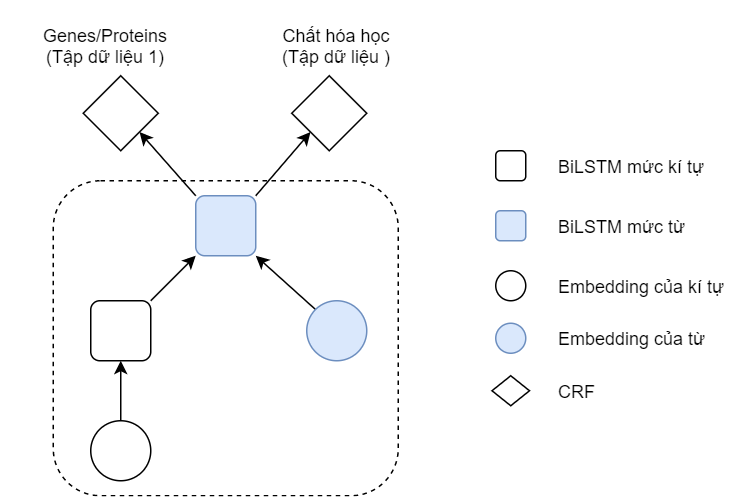
\includegraphics[scale=0.4]{03-multitask}
\caption{Mô hình học đa tác vụ. Hình tròn màu trắng thể hiện embedding của các kí tự. Hình chữ nhật có viền tròn thể hiện thông tin về kí tự khi đi qua BiLSTM. Hình tròn có màu xanh thể hiện embedding ở mức từ. Hình chữ nhật viền tròn có màu xanh thể hiện thông tin ở mức từ khi đi qua BiLSTM. Hình vuông thể hiện lớp CRF. Tham số về từ và kí tự được sử dụng chung cho tất cả các tác vụ}
\end{figure}

\end{document}